\section{Materials and Methods}
\label{sec:methods}

\subsection{System overview}
Fig.~\ref{fig:pipeline} shows the pipeline. Components in the top row prepare data; the adapter was trained once in the joint session; everything in the lower row is ours and runs on CPU.
\begin{figure}[t]\centering
\resizebox{\columnwidth}{!}{\begin{tikzpicture}[node distance=4mm and 5mm, box/.style={draw,rounded corners,align=center,font=\scriptsize,minimum height=7mm,inner sep=2pt,text width=1.55cm}, arr/.style={-{Latex[length=1.6mm]}}]
\node[box] (d) {TrialGPT annotations};
\node[box,right=of d] (s) {Patient-grouped split 37/8/8};
\node[box,right=of s] (p) {Prompt contract + SFT encode};
\node[box,below=of p] (l) {LoRA adapter (joint GPU run)};
\node[box,left=of l] (m) {Qwen2.5-1.5B base};
\node[box,left=of m] (e) {Eval: label, evidence, errors};
\node[box,below=of e] (k) {KV-cache decoder + tiled attention};
\node[box,right=of k] (sp) {Speculative decoder (0.5B draft)};
\node[box,right=of sp] (a) {Kormat web app};
\draw[arr] (d)--(s); \draw[arr] (s)--(p); \draw[arr] (p)--(l); \draw[arr] (m)--(l);
\draw[arr] (m)--(e); \draw[arr] (e)--(k); \draw[arr] (k)--(sp); \draw[arr] (sp)--(a);
\end{tikzpicture}
}
\caption{System pipeline: data preparation, adapted model, evaluation, own inference stack, application.}
\label{fig:pipeline}
\end{figure}

\subsection{Dataset and split}
\label{sec:dataset}
We use only the NCBI TrialGPT criterion annotations~\cite{trialgpt_criterion_annotations}: 1{,}015 criterion annotations for 53 patients, each with a patient description, criterion type and text, expert label and expert evidence sentence IDs. The dataset also contains GPT-4 predictions and explanations; these are never used as input or in evaluation. Unique patient IDs are sorted, shuffled with \texttt{numpy.random.default\_rng(42)}, and the first 37 go to training, the next 8 to validation and the last 8 to test; every annotation of a patient lies in exactly one split. The manifest is saved in \texttt{results/split\_manifest.json} and a leakage check asserts empty pairwise patient intersections. The test split was untouched until final evaluation.
\maybeinput{tables/data_stats} Fig.~\ref{fig:labels} shows the label distribution. % TODO-INTERPRET: split sizes, class imbalance
\begin{figure}[t]\centering
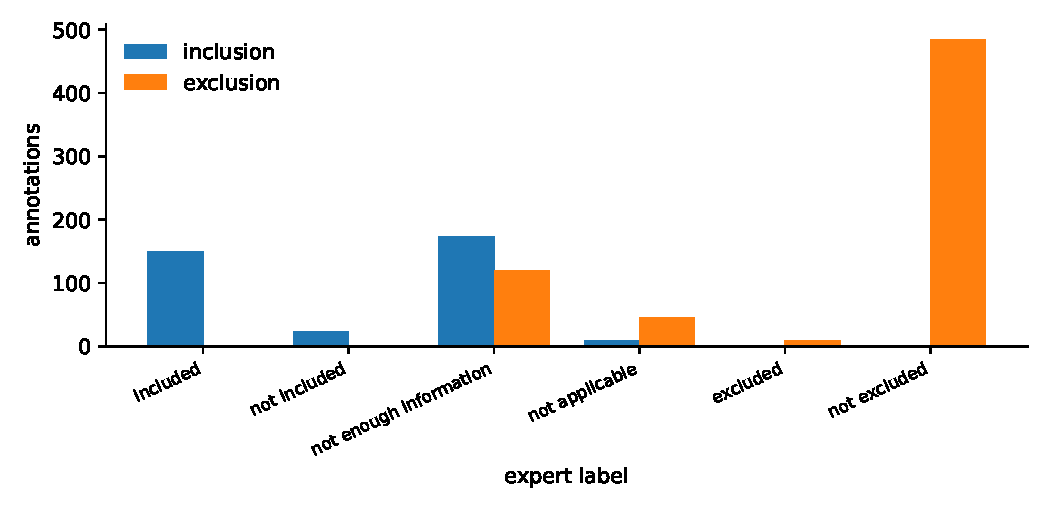
\includegraphics[width=\columnwidth]{figures/label_distribution.pdf}
\caption{Label distribution per criterion type and split.}
\label{fig:labels}
\end{figure}
% TODO-INTERPRET: Fig. labels: class imbalance, which classes are rare, consequence for macro-F1.

\subsection{Input/output processing and tokenization}
\label{sec:io}
Each patient note is split into numbered sentences following the dataset's sentence indexing. A single prompt contract (system message, numbered note, criterion type, criterion, allowed labels, JSON return format) is shared by training, evaluation, benchmarks and the app, so all see the identical string. The target is a JSON object \texttt{\{"label": ..., "evidence": [ids]\}}; the label set depends on criterion type and is never collapsed to yes/no. Text is tokenised with the Qwen2.5 tokenizer (151{,}936 tokens, identical for the 1.5B and 0.5B models) through the chat template. Training examples longer than 1{,}024 tokens are dropped, never cut mid-text, so no relevant evidence is silently removed.
\maybeinput{tables/token_lengths} Fig.~\ref{fig:toklen} shows the length distribution. % TODO-INTERPRET: number dropped per split, any evidence lost.
\begin{figure}[t]\centering
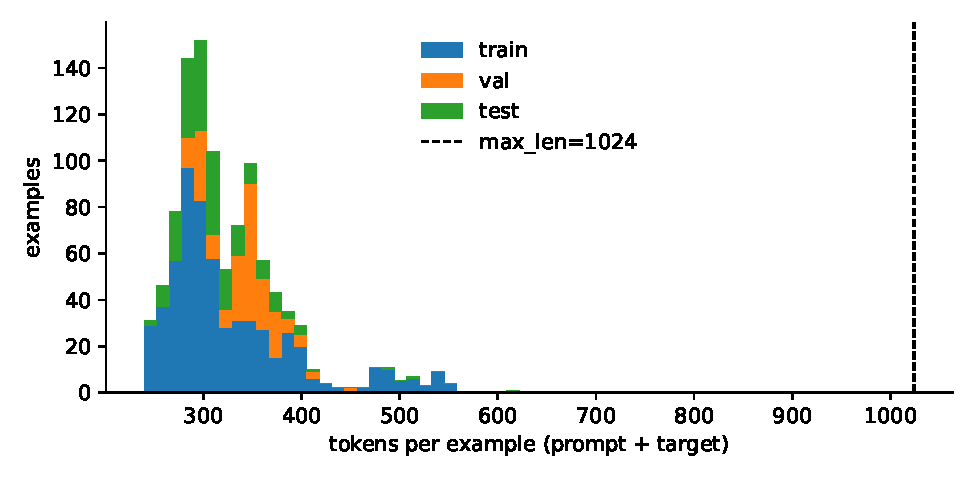
\includegraphics[width=\columnwidth]{figures/token_lengths.pdf}
\caption{Prompt length in tokens per split with the truncation threshold.}
\label{fig:toklen}
\end{figure}

\subsection{Model selection}
\label{sec:model}
Table~\ref{tab:models} compares four open-weight decoder candidates using the \texttt{config.json} files on the Hugging Face Hub (Llama-3.2-1B is gated, so its figures come from a public mirror). We chose Qwen2.5-1.5B-Instruct~\cite{qwen2024qwen25}: 28 layers, hidden size 1536, 12 query heads and 2 KV heads with head dimension 128, 32{,}768-token context, Apache-2.0, and a KV cache of 28{,}672 bytes per token in bf16, 6.9$\times$ smaller than the multi-head SmolLM2-1.7B. Qwen2.5-0.5B-Instruct shares its tokenizer (identical vocabulary, merges, special tokens, chat template; zero id mismatches on 50 test strings) and serves as the draft model. The base was fixed by the shared training run; we did not fine-tune the other candidates and make no claim that Qwen2.5 beats them.
\begin{table}[t]
\caption{Candidate open decoder models (config.json; memory by arithmetic, GiB).}
\label{tab:models}
\centering\scriptsize
\begin{tabular}{@{}lrrrr@{}}
\toprule
 & Qwen2.5-1.5B & Qwen3-1.7B & Llama-3.2-1B$^{\ast}$ & SmolLM2-1.7B \\
\midrule
Params (B) & 1.54 & 2.03$^{\dagger}$ & 1.24 & 1.71 \\
Layers & 28 & 28 & 16 & 24 \\
Hidden & 1536 & 2048 & 2048 & 2048 \\
Heads Q/KV & 12/2 & 16/8 & 32/8 & 32/32 \\
head\_dim & 128 & 128 & 64 & 64 \\
Vocab & 151,936 & 151,936 & 128,256 & 49,152 \\
Context & 32,768 & 40,960 & 131,072 & 8,192 \\
RoPE $\theta$ & $10^6$ & $10^6$ & $5\!\times\!10^5$ & 130,000 \\
Licence & Apache-2.0 & Apache-2.0 & Llama 3.2 & Apache-2.0 \\
fp32 / bf16 / 4-bit & 5.75/2.88/0.72 & 7.57/3.78/0.95 & 4.60/2.30/0.58 & 6.38/3.19/0.80 \\
KV B/token (bf16) & 28,672 & 114,688 & 32,768 & 196,608 \\
\bottomrule
\end{tabular}\\[2pt]
{\scriptsize $^{\ast}$ gated; values from public mirror. $^{\dagger}$ safetensors total incl.\ embeddings (card: 1.7B).}
\end{table}
% TODO-INTERPRET: Table models: GQA drives the KV-bytes column; why CPU RAM (15 GB) rules out larger caches; weights fit.

\subsection{Fine-tuning}
\label{sec:finetune}
\textbf{Disclosure.} The LoRA adapter was trained in a \emph{joint session} on a shared GPU with M.\ Ruhan Kamran (23i-0062) and published as \texttt{arceus1rk/eligitrace-qwen2.5-1.5b-lora}. We did not train it alone; we use it, and all evaluation, inference code and application are our own, run on a CPU laptop.

\textbf{Method choice.} For $N=1.54\times10^9$ parameters, full fine-tuning with mixed-precision AdamW needs about $16N\approx 23$~GiB for weights, gradients and optimiser state; LoRA~\cite{hu2022lora} with $r{=}16$ on $q,k,v,o,\mathrm{gate},\mathrm{up},\mathrm{down}$ trains 18{,}464{,}768 parameters (1.2\%), about 3.1~GiB in total; QLoRA~\cite{dettmers2023qlora} would reach about 1.0~GiB but adds quantisation overhead unnecessary at this size. Prompt-only is our ``before'' baseline.

\textbf{Configuration.} LoRA $r=16$, $\alpha=32$, dropout 0.05, 3 epochs, learning rate $2\times10^{-4}$ with cosine schedule, effective batch size 16, bf16. The training objective is next-token cross-entropy on the assistant JSON only (prompt tokens masked). % TODO-INTERPRET: confirm masking, warmup, seed, steps and curves from the shared run record; add training-curve figure in Results.

\subsection{Own KV-cache decoder}
\label{sec:kv}
We implement a per-layer pre-allocated buffer of shape (batch, KV heads, max length, head dim) and one integer \texttt{length}. Prefill writes all prompt keys and values (already RoPE-rotated) once; each decode step writes one position and attends to the view \texttt{buf[..., :length, :]}. Compared with concatenating tensors each step (copy cost $O(n)$ per token), a slice write is $O(1)$ in cache size, and rollback needed by speculative decoding only moves the integer (Fig.~\ref{fig:kv}). Cache size follows $2\cdot L\cdot n_{kv}\cdot d_h\cdot b$ bytes per token.
\begin{figure}[t]\centering
\resizebox{\columnwidth}{!}{\begin{tikzpicture}[node distance=4mm, box/.style={draw,rounded corners,align=center,font=\scriptsize,minimum height=6.5mm,text width=1.7cm,inner sep=2pt}, arr/.style={-{Latex[length=1.6mm]}}]
\node[box] (pf) {Prefill: all $n$ prompt tokens};
\node[box,right=of pf] (w) {Write K,V to \texttt{buf[:, :, 0:n]}};
\node[box,right=of w] (dec) {Decode: 1 token, attend to \texttt{buf[:len]}};
\node[box,below=of dec] (app) {Append K,V at \texttt{len}; \texttt{len}$\mathrel{+}=1$};
\node[box,left=of app] (rb) {Rollback: \texttt{crop(len')} moves the integer only};
\draw[arr] (pf)--(w); \draw[arr] (w)--(dec); \draw[arr] (dec)--(app); \draw[arr] (app)--(rb);
\draw[arr] (app.south) -- ++(0,-4mm) -| node[pos=.25,below,font=\scriptsize]{next token} (dec.south east);
\end{tikzpicture}
}
\caption{Prefill and decode flow of the pre-allocated KV cache, with O(1) rollback.}
\label{fig:kv}
\end{figure}

\subsection{Tiled online-softmax attention}
\label{sec:attn}
For one head, $O=\mathrm{softmax}(QK^\top/\sqrt{d})V$. Following the online normaliser~\cite{milakov2018online} and its tiled use~\cite{rabe2021selfattention,dao2022flashattention}, we iterate over key blocks keeping a running row maximum $m$, normaliser $l$ and unnormalised output $O$ (Fig.~\ref{fig:tile}, Algorithm~\ref{alg:tiled}). The $L\times L$ matrix is never formed; only $B_q\times B_k$ tiles are. Accumulation is in fp32. Masks (causal, padding) are applied per tile; fully masked rows return zero and guard against $-\infty-(-\infty)$.
\begin{figure}[t]\centering
\resizebox{\columnwidth}{!}{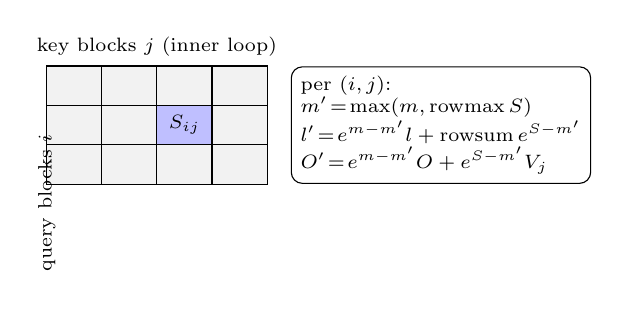
\begin{tikzpicture}[font=\scriptsize]
\foreach \i in {0,1,2} \foreach \j in {0,1,2,3} {
  \draw[fill=gray!10] (\j*0.7,-\i*0.5) rectangle ++(0.7,-0.5);
}
\draw[fill=blue!25] (1.4,-0.5) rectangle ++(0.7,-0.5);
\node at (1.75,-0.75) {$S_{ij}$};
\node[above] at (1.4,0) {key blocks $j$ (inner loop)};
\node[rotate=90,left] at (0,-0.75) {query blocks $i$};
\node[draw,rounded corners,align=left,right] at (3.1,-0.75) {per $(i,j)$:\\ $m'\!=\!\max(m,\mathrm{rowmax}\,S)$\\ $l'\!=\!e^{m-m'}l+\mathrm{rowsum}\,e^{S-m'}$\\ $O'\!=\!e^{m-m'}O+e^{S-m'}V_j$};
\end{tikzpicture}
}
\caption{Tile loop: for each query block, scan key blocks and update $(m,l,O)$.}
\label{fig:tile}
\end{figure}
\begin{algorithm}[t]
\caption{Tiled online-softmax attention (one head)}
\label{alg:tiled}
\begin{algorithmic}[1]
\Require $Q\in\mathbb{R}^{L_q\times d}$, $K,V\in\mathbb{R}^{L_k\times d}$, block sizes $B_q,B_k$, mask $M$
\For{each query block $Q_i$ ($B_q$ rows)}
  \State $m\gets -\infty,\; l\gets 0,\; O\gets 0$
  \For{each key block $(K_j,V_j)$}
    \State $S\gets Q_iK_j^\top/\sqrt{d}$; apply mask $M_{ij}$
    \State $m'\gets\max(m,\mathrm{rowmax}(S))$
    \State $P\gets \exp(S-m')$
    \State $l\gets e^{m-m'}\,l+\mathrm{rowsum}(P)$
    \State $O\gets e^{m-m'}\,O+PV_j$;\quad $m\gets m'$
  \EndFor
  \State output rows $O_i\gets O/l$
\EndFor
\end{algorithmic}
\end{algorithm}
We validate against the reference softmax attention (max absolute difference, and equality of generated tokens), see Sec.~\ref{sec:results}. Because the speed-ups reported for this family of methods come from GPU memory hierarchy~\cite{dao2022flashattention}, we expect memory savings on CPU but not necessarily speed-ups, and test this.

\subsection{Greedy speculative decoding}
\label{sec:spec}
We implement greedy speculative decoding~\cite{leviathan2023speculative,chen2023speculative}: the 0.5B draft proposes $k$ tokens, the 1.5B target scores prefix plus proposals in a single forward pass, and the longest prefix on which draft and target argmax agree is accepted; the target's own next token is appended. Both caches roll back to the accepted length (Fig.~\ref{fig:spec}, Algorithm~\ref{alg:spec}). With greedy acceptance the output is token-identical to greedy decoding of the target, which we verify.
\begin{figure}[t]\centering
\resizebox{\columnwidth}{!}{\begin{tikzpicture}[node distance=4mm, box/.style={draw,rounded corners,align=center,font=\scriptsize,minimum height=6.5mm,text width=1.7cm,inner sep=2pt}, arr/.style={-{Latex[length=1.6mm]}}]
\node[box] (d) {Draft 0.5B proposes $k$ tokens greedily};
\node[box,right=of d] (v) {Target 1.5B scores prefix + $k$ in one pass};
\node[box,right=of v] (c) {Accept longest matching prefix};
\node[box,below=of c] (r) {Rollback both caches to accepted length};
\node[box,left=of r] (b) {Append target's own next token};
\draw[arr] (d)--(v); \draw[arr] (v)--(c); \draw[arr] (c)--(r); \draw[arr] (r)--(b);
\draw[arr] (b.west) -- ++(-3mm,0) |- (d.west);
\end{tikzpicture}
}
\caption{Draft, verify and rollback loop of speculative decoding.}
\label{fig:spec}
\end{figure}
\begin{algorithm}[t]
\caption{Greedy speculative decoding}
\label{alg:spec}
\begin{algorithmic}[1]
\Require target $T$, draft $D$ (same tokenizer), prompt $x$, draft length $k$, max new tokens $N$
\State prefill caches of $T$ and $D$ with $x$; $y\gets[\,]$
\While{$|y|<N$ and no EOS}
  \State $d_1..d_k\gets$ greedy decode of $D$ (each step uses $D$'s cache)
  \State $t_0..t_k\gets \arg\max$ of $T$ logits on $[\text{last},d_1..d_k]$ (one pass)
  \State $a\gets$ largest $a\le k$ with $d_i=t_{i-1}$ for all $i\le a$
  \State append $d_1..d_a$ and $t_a$ to $y$
  \State roll back caches of $T$ and $D$ to the verified prefix (discard rejected positions)
\EndWhile
\State \Return $y$
\end{algorithmic}
\end{algorithm}

\subsection{Application workflow}
\label{sec:app}
``Kormat'' is a FastAPI service with a static browser front end. A user pastes a patient description and one or more criteria; the server splits sentences, builds the shared prompt, decodes (with cache and optional speculation), parses and validates the JSON (cited IDs must exist in the note), and returns per-criterion label, cited IDs, evidence text and an explanation based only on the note (Fig.~\ref{fig:app}). Multiple criteria may be combined into a patient--trial summary by explicit rules, which is an aggregation and not a ground-truth outcome. % TODO-INTERPRET: add rule table and screenshots (figures/app_*.png) when TGA-36..41 land.
\begin{figure}[t]\centering
\resizebox{\columnwidth}{!}{\begin{tikzpicture}[node distance=4mm, box/.style={draw,rounded corners,align=center,font=\scriptsize,minimum height=6.5mm,text width=1.7cm,inner sep=2pt}, arr/.style={-{Latex[length=1.6mm]}}]
\node[box] (u) {Browser: note + criteria};
\node[box,right=of u] (api) {FastAPI endpoint};
\node[box,right=of api] (sp) {Sentence split + prompt};
\node[box,below=of sp] (g) {Decode (cache/spec.)};
\node[box,left=of g] (pa) {Parse JSON, validate IDs};
\node[box,left=of pa] (ag) {Rule-based aggregation};
\draw[arr] (u)--(api); \draw[arr] (api)--(sp); \draw[arr] (sp)--(g); \draw[arr] (g)--(pa); \draw[arr] (pa)--(ag);
\draw[arr] (ag.north) -- ++(0,4mm) -| (u.south);
\end{tikzpicture}
}
\caption{Application request flow.}
\label{fig:app}
\end{figure}
